% \begin{frame}
%   {Kernfragen dieser Woche}
%   \onslide<+->
%   \onslide<+->
%   \Large
%   \centering 
%   Verständnis dafür, dass wir bisher nur über \alert{Extensionen} sprechen.\\
%   \Halbzeile
%   \onslide<+->
%   Wissen um Konstruktionen, in denen das nicht ausreicht.\\
%   \Halbzeile
%   \onslide<+->
%   Definition des intensionalen Kalküls auf Basis des extensionalen.\\
%   \Halbzeile
%   \onslide<+->
%   Nochmals zurück zu Chierchia,\\
%   weil das entsprechende Kapitel wirklich gut ist.\\
%   \onslide<+->
%   \Halbzeile
%   \grau{\footnotesize Texte für heute: \citealt[Kapitel~5]{ChierchiaMcconnellginet2000} | \citet[Kapitel~5--6]{DowtyEa1981}}
% \end{frame}

\section{Intensionalität und Modallogik}

\subsection{Wozu Intensionalität?}

\begin{frame}
  {Intensionalität | Beispiele}
  \onslide<+->
  \begin{itemize}[<+->]
    \item \textit{Stockhausen \alert{wird} eine andere Oper schreiben.}
    \item \textit{\alert{Hätte} Arno Schmidt weniger getrunken, \alert{könnte} er noch leben.}
    \item \textit{Gustave Moreau \alert{glaubt}, dass Ästhetizismus toll ist.}
  \end{itemize}
\end{frame}

\begin{frame}
  {Probleme mit Extensionen}
  \onslide<+->
  \onslide<+->
  \begin{itemize}
    \item \grau{\textit{Stockhausen {wird} eine andere Oper schreiben.}}
    \item \grau{\textit{{Hätte} Arno Schmidt weniger getrunken, {könnte} er noch leben.}}
    \item \grau{\textit{Gustave Moreau {glaubt}, dass Ästhetizismus toll ist.}}
  \end{itemize}
  \Halbzeile
  \begin{itemize}[<+->]
    \item \alert{Syntax} der Ausdrücke | Problemlos mit Einführung von Auxiliaren
    \item \alert{Wahrheitsbedingungen} | \rot{Nicht angebbar}
      \begin{itemize}[<+->]
        \item in eindimensionalen Modellen ohne Tempus 
        \item und ohne Modellierung von Möglichkeit und Notwendigkeit\\
          \grau{\footnotesize(Modalverben, modale Adverbiale, \textit{glauben}-Verben)}
      \end{itemize}
  \end{itemize}
\end{frame}


\begin{frame}
  {Was sind Intensionen?}
  \onslide<+->
  \onslide<+->
  \gruen{Extension} (Bedeutung) und \alert{Intension} (Sinn)\\
  \onslide<+->
  \Zeile
  \centering 
  \begin{tabular}{llll}
    \toprule
    \textbf{Synt.\ Typ} & \textbf{Bedeutung} & \textbf{Sinn} & \textbf{Beispiele} \\
    \midrule
    \visible<4->{NP & \gruen<4>{Individuum} & \alert<4>{Individuenkonzept} & \emph{Venus}, \textit{Helmut Kohl}} \\
    \visible<5->{VP & \gruen<5>{Menge von Individuen} & \alert<5>{Eigenschaftskonzept} & \emph{Kolibri}, \textit{laufen}} \\
    \visible<6->{S  & \gruen{Wahrheitswert} & \alert{Proposition} \grau{(Gedanke)} & \emph{Ich mag Kolibris.} }\\
    \bottomrule
  \end{tabular}
\end{frame}

\begin{frame}
  {Intensionen}
  \onslide<+->
  \onslide<+->
  Noch wissen wir nicht viel über Intensionen. Offensichtliche Eigenschaften aber:\\
  \Halbzeile
  \begin{itemize}[<+->]
    \item Nicht rein wahrheitsfunktional in der wirklichen jetzigen Welt\\
      \grau{\footnotesize "`Was ist in der Welt der Fall?"' reicht nicht aus.}
    \item Wissen über die \alert{tatsächlichen}, \alert{vergangenen} und \alert{möglichen} Zustände der Welt\\
      \grau{\footnotesize PSOA = \textit{possible state of affairs}}\\
      \grau{\footnotesize Z.\,B.\ alle vergangenen SOAs; die PSOAs, die Horst Lichter für möglich hält usw.}
    \item Sowas wie \alert{mehrdimensionale Wahrheitsbedingungen}
    \item Vermitteln zwischen Wissen über Dinge und Wahrheitswerten
  \end{itemize}
\end{frame}

\begin{frame}
  {Logik von PSOAs}
  \onslide<+->
  \onslide<+->
  Wir brauchen eine Logik für PSOAs!\\
  \Halbzeile
  \begin{itemize}[<+->]
    \item Offensichtliche \alert{logische Beschränkungen auf PSOAs}
      \Halbzeile
    \item Solche Sätze scheitern nicht nur, weil sie nicht wahr sind:\\
      \alert{\textit{Im Jahr 1985 wird Arno Schmidt planen, "`\textit{Julia}"' bis 1914 fertig zu schreiben.}}
      \Halbzeile
    \item \orongsch{Inkompatibel} mit unserem Wissen über \orongsch{zulässige\slash mögliche PSOAs}
  \end{itemize}
\end{frame}

\begin{frame}
  {Paralleluniversen?}
  \onslide<+->
  \onslide<+->
  \alert{\textit{Maria könnte Arno Schmidt persönlich kennen.}}\\
  \Zeile
  \begin{itemize}[<+->]
    \item Realität | Maria wurde nach dem Tod von AS geboren.
      \Halbzeile
    \item Vorstellbare alternative Realitäten
      \begin{enumerate}[<+->]
        \item AS ist kein Workaholic, trinkt nicht eine Flasche Korn am Tag\\
          und hat daher 1979 keinen Infarkt.
        \item Maria wurde zwanzig Jahre früher geboren.
        \item AS ist von den Toten auferstanden.
        \item \grau{Im Prinzip unbegrenzt viele Möglichkeiten}
      \end{enumerate}
  \end{itemize}
\end{frame}

\subsection{Formale Modellierung von Intensionen}

\begin{frame}
  {Propositionen und PSOAs}
  \onslide<+->
  \onslide<+->
  Basis der Formalisierung\\
  \Halbzeile
  \begin{itemize}[<+->]
    \item Annahme einer \alert{Menge von PSOAs} (= mögliche Welten)
      \Halbzeile
    \item Jeder PSOA | Exhaustiv bestimmt durch die in ihm wahren Propositionen
      \Halbzeile
    \item Jede Proposition | Zwei-Partitionierung der PSOAs:
      \begin{itemize}[<+->]
        \item Die, in denen sie \alert{wahr} ist
        \item Die, in denen sie \orongsch{falsch} ist
      \end{itemize}
  \end{itemize}
\end{frame}

\begin{frame}
  {Mögliche Welten und Zeiten in Koordinaten}
  \onslide<+->
  \begin{itemize}[<+->]
    \item Für jede \gruen{Proposition} $p_n$ | \gruen{Welten, in der $\dem{p_n}=1$} | \alert{$w\in W$}
    \item Für jeden \gruen{Zeitpunkt} | Ein möglicher Zustand jeder Welt | \alert{$i\in I$}
    \item Also zeitlich geordnete \gruen{Welt-Zeit-Koordinaten} | \alert{$\langle w, i\rangle\in W\times I$}
  \end{itemize}
  \Zeile
  \centering
  \onslide<+->
  \resizebox{0.4\textwidth}{!}{
    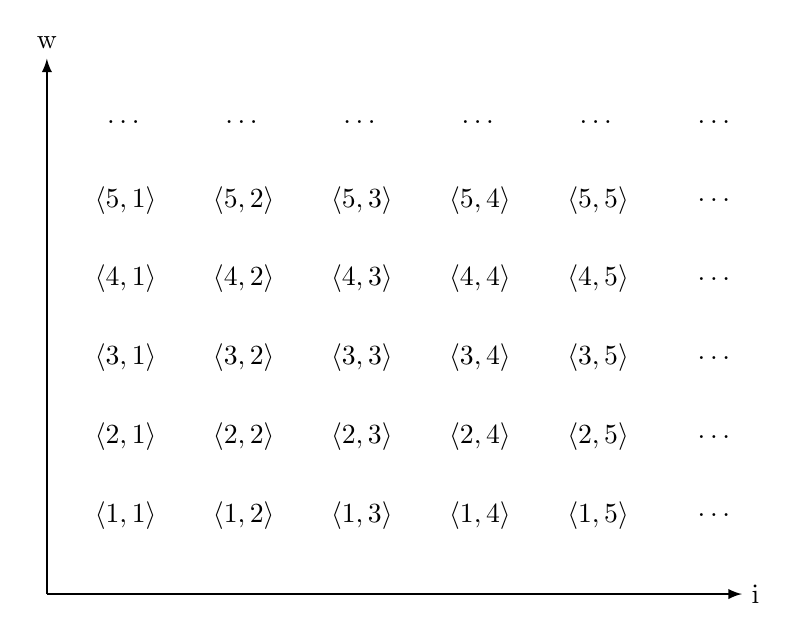
\begin{tikzpicture}

      \node (w) at (0, 7) {w};
      \node (i) at (9, 0) {i};
      \path (0, 0) edge [line width=0.25mm, -latex] (w);
      \path (0, 0) edge [line width=0.25mm, -latex] (i);

      \node [] (w11) at (1, 1) {${\langle 1,1\rangle}$};
      \node [] (w21) at (1, 2) {${\langle 2,1\rangle}$};
      \node [] (w31) at (1, 3) {${\langle 3,1\rangle}$};
      \node [] (w41) at (1, 4) {${\langle 4,1\rangle}$};
      \node [] (w51) at (1, 5) {${\langle 5,1\rangle}$};
      \node [] (w61) at (1, 6) {\ldots};

      \node [] (w12) at (2.5, 1) {${\langle 1,2\rangle}$};
      \node [] (w22) at (2.5, 2) {${\langle 2,2\rangle}$};
      \node [] (w32) at (2.5, 3) {${\langle 3,2\rangle}$};
      \node [] (w42) at (2.5, 4) {${\langle 4,2\rangle}$};
      \node [] (w52) at (2.5, 5) {${\langle 5,2\rangle}$};
      \node [] (w62) at (2.5, 6) {\ldots};

      \node [] (w13) at (4, 1) {${\langle 1,3\rangle}$};
      \node [] (w23) at (4, 2) {${\langle 2,3\rangle}$};
      \node [] (w33) at (4, 3) {${\langle 3,3\rangle}$};
      \node [] (w43) at (4, 4) {${\langle 4,3\rangle}$};
      \node [] (w53) at (4, 5) {${\langle 5,3\rangle}$};
      \node [] (w63) at (4, 6) {\ldots};

      \node [] (w14) at (5.5, 1) {${\langle 1,4\rangle}$};
      \node [] (w24) at (5.5, 2) {${\langle 2,4\rangle}$};
      \node [] (w34) at (5.5, 3) {${\langle 3,4\rangle}$};
      \node [] (w44) at (5.5, 4) {${\langle 4,4\rangle}$};
      \node [] (w54) at (5.5, 5) {${\langle 5,4\rangle}$};
      \node [] (w64) at (5.5, 6) {\ldots};

      \node [] (w15) at (7, 1) {${\langle 1,5\rangle}$};
      \node [] (w25) at (7, 2) {${\langle 2,5\rangle}$};
      \node [] (w35) at (7, 3) {${\langle 3,5\rangle}$};
      \node [] (w45) at (7, 4) {${\langle 4,5\rangle}$};
      \node [] (w55) at (7, 5) {${\langle 5,5\rangle}$};
      \node [] (w65) at (7, 6) {\ldots};

      \node [] (w16) at (8.5, 1) {\ldots};
      \node [] (w26) at (8.5, 2) {\ldots};
      \node [] (w36) at (8.5, 3) {\ldots};
      \node [] (w46) at (8.5, 4) {\ldots};
      \node [] (w56) at (8.5, 5) {\ldots};
      \node [] (w66) at (8.5, 6) {\ldots};
    \end{tikzpicture}
  }
\end{frame}

\begin{frame}
  {Propositionen und Welten}
  \onslide<+->
  \onslide<+->
  Propositionen sind die Intensionen von Formeln bzw.\ Sätzen!\\
  \Halbzeile
  \begin{itemize}[<+->]
    \item Maximal alle Welten für jede Proposition als wahr, permutiert mit allen anderen\\
      \grau{\footnotesize $w_1$: $p_1$ wahr, alle anderen $p_n$ falsch}\\
      \grau{\footnotesize $w_{12}$: $p_1$ und $p_2$ wahr, alle anderen $p_n$ falsch}\\
      \grau{\footnotesize $w_2$: $p_2$ wahr, alle anderen $p_n$ falsch usw.}\\
    \item Exhaustive Charakterisierung eines Satzes | \alert{Alle Welten, in denen er wahr ist}
    \item \gruen{Intension eines Satzes} | \alert{Alle Welten, in denen er wahr ist}
      \Halbzeile
    \item \gruen{Proposition eines Satzes} | \alert{Charakteristische Funktion} der Menge\\
      der \alert{Welten, in denen er wahr ist} \grau{zu den Zeitpunkten, zu denen er wahr ist}
  \end{itemize}
\end{frame}

\begin{frame}
  {Propositionen als Funktionen}
  \onslide<+->
  \onslide<+->
  Propositionen sind \alert{Funktionen $\{0,1\}^{W\times I}$}\\
  \Zeile
  \onslide<+->
  \centering 
  \resizebox{0.4\textwidth}{!}{
    \begin{tikzpicture}

      \node [rectangle, draw, align=left, color=teal, rounded corners=0.5em] (T) at (4.5, 8) {\Huge 1};
      \node [rectangle, draw, align=left, color=orongsch, rounded corners=0.5em] (F) at (3.5, -2) {\Huge 0};

      \node (w) at (0, 7) {w};
      \node (i) at (9, 0) {i};
      \path (0, 0) edge [line width=0.25mm, -latex] (w);
      \path (0, 0) edge [line width=0.25mm, -latex] (i);

      \node [color=teal] (w11) at (1, 1) {${\langle 1,1\rangle}$};
      \node [color=orongsch] (w21) at (1, 2) {${\langle 2,1\rangle}$};
      \node [color=teal] (w31) at (1, 3) {${\langle 3,1\rangle}$};
      \node [color=orongsch] (w41) at (1, 4) {${\langle 4,1\rangle}$};
      \node [color=orongsch] (w51) at (1, 5) {${\langle 5,1\rangle}$};
      \node [color=gray] (w61) at (1, 6) {\ldots};

      \path (w11) edge [line width=0.2mm, -latex, color=teal] (T);
      \path (w21) edge [line width=0.2mm, -latex, color=orongsch] (F);
      \path (w31) edge [line width=0.2mm, -latex, color=teal] (T);
      \path (w41) edge [line width=0.2mm, -latex, color=orongsch] (F);
      \path (w51) edge [line width=0.2mm, -latex, color=orongsch] (F);

      \node [color=orongsch] (w12) at (2.5, 1) {${\langle 1,2\rangle}$};
      \node [color=orongsch] (w22) at (2.5, 2) {${\langle 2,2\rangle}$};
      \node [color=orongsch] (w32) at (2.5, 3) {${\langle 3,2\rangle}$};
      \node [color=orongsch] (w42) at (2.5, 4) {${\langle 4,2\rangle}$};
      \node [color=teal] (w52) at (2.5, 5) {${\langle 5,2\rangle}$};
      \node [color=gray] (w62) at (2.5, 6) {\ldots};

      \path (w12) edge [line width=0.2mm, -latex, color=orongsch] (F);
      \path (w22) edge [line width=0.2mm, -latex, color=orongsch] (F);
      \path (w32) edge [line width=0.2mm, -latex, color=orongsch] (F);
      \path (w42) edge [line width=0.2mm, -latex, color=teal] (T);
      \path (w52) edge [line width=0.2mm, -latex, color=teal] (T);

      \node [color=teal] (w13) at (4, 1) {${\langle 1,3\rangle}$};
      \node [color=orongsch] (w23) at (4, 2) {${\langle 2,3\rangle}$};
      \node [color=teal] (w33) at (4, 3) {${\langle 3,3\rangle}$};
      \node [color=orongsch] (w43) at (4, 4) {${\langle 4,3\rangle}$};
      \node [color=teal] (w53) at (4, 5) {${\langle 5,3\rangle}$};
      \node [color=gray] (w63) at (4, 6) {\ldots};

      \path (w13) edge [line width=0.2mm, -latex, color=teal] (T);
      \path (w23) edge [line width=0.2mm, -latex, color=orongsch] (F);
      \path (w33) edge [line width=0.2mm, -latex, color=teal] (T);
      \path (w43) edge [line width=0.2mm, -latex, color=orongsch] (F);
      \path (w53) edge [line width=0.2mm, -latex, color=teal] (T);

      \node [color=orongsch] (w14) at (5.5, 1) {${\langle 1,4\rangle}$};
      \node [color=teal] (w24) at (5.5, 2) {${\langle 2,4\rangle}$};
      \node [color=teal] (w34) at (5.5, 3) {${\langle 3,4\rangle}$};
      \node [color=orongsch] (w44) at (5.5, 4) {${\langle 4,4\rangle}$};
      \node [color=orongsch] (w54) at (5.5, 5) {${\langle 5,4\rangle}$};
      \node [color=gray] (w64) at (5.5, 6) {\ldots};

      \path (w14) edge [line width=0.2mm, -latex, color=orongsch] (F);
      \path (w24) edge [line width=0.2mm, -latex, color=teal] (T);
      \path (w34) edge [line width=0.2mm, -latex, color=teal] (T);
      \path (w44) edge [line width=0.2mm, -latex, color=orongsch] (F);
      \path (w54) edge [line width=0.2mm, -latex, color=orongsch] (F);

      \node [color=orongsch] (w15) at (7, 1) {${\langle 1,5\rangle}$};
      \node [color=teal] (w25) at (7, 2) {${\langle 2,5\rangle}$};
      \node [color=orongsch] (w35) at (7, 3) {${\langle 3,5\rangle}$};
      \node [color=orongsch] (w45) at (7, 4) {${\langle 4,5\rangle}$};
      \node [color=orongsch] (w55) at (7, 5) {${\langle 5,5\rangle}$};
      \node [color=gray] (w65) at (7, 6) {\ldots};

      \path (w15) edge [line width=0.2mm, -latex, color=orongsch] (F);
      \path (w25) edge [line width=0.2mm, -latex, color=teal] (T);
      \path (w35) edge [line width=0.2mm, -latex, color=orongsch] (F);
      \path (w45) edge [line width=0.2mm, -latex, color=orongsch] (F);
      \path (w55) edge [line width=0.2mm, -latex, color=teal] (T);

      \node [color=gray] (w16) at (8.5, 1) {\ldots};
      \node [color=gray] (w26) at (8.5, 2) {\ldots};
      \node [color=gray] (w36) at (8.5, 3) {\ldots};
      \node [color=gray] (w46) at (8.5, 4) {\ldots};
      \node [color=gray] (w56) at (8.5, 5) {\ldots};
      \node [color=gray] (w66) at (8.5, 6) {\ldots};
    \end{tikzpicture}
  }
\end{frame}


\begin{frame}
  {Überlegen Sie sich das mal \ldots}
  \onslide<+->
  Sind solche Propositionen als Intensionen wirklich \rot{un}befriedigend?\\
  \Halbzeile
  \begin{itemize}[<+->]
    \item Wenn wir den \alert{aktuellen SOA exhaustiv} kennen,\\
      wissen wir für \gruen{jeden Satz, ob er wahr ist}.
      \Halbzeile
    \item Wenn wir wissen, \gruen{welche Sätze wahr sind},\\
      kennen wir den \alert{aktuellen SOA exhaustiv}.
      \Halbzeile
    \item Sätze denotieren Wahrheitswerte, und die Wahrheit eines Satzes\\
      hängt nur vom aktuellem SOA ab.
      \Viertelzeile
    \item[ ] \gruen{Eine Funktion von möglichen Welten zu Wahrheitswerten}\\
      \gruen{charakterisiert daher die Semantik eines Satzes umfassend.}
      \Viertelzeile
    \item Was mehr gäbe es über einen Satz zu wissen?
    \item \orongsch{Sätze mit derselben Intension $\{0,1\}^{W\times I}$ sind absolut gleichbedeutend.}
  \end{itemize}
\end{frame}


\subsection{Mengen von Welten}

\begin{frame}
  {Implikation und Welten}
  \onslide<+->
  \onslide<+->
  Satzintensionen | Charakteristische Funktionen -- oder \alert{Mengen von $w$ bzw.\ $\langle w,i \rangle$}\\
  \onslide<+->
  \Zeile
  \centering 
  $\alert{p}\rightarrow \gruen{q}$ entspricht $\alert{P}\subseteq \gruen{Q}$:\\
  \Halbzeile
  \onslide<+->
  \resizebox{0.4\textwidth}{!}{
    \begin{tikzpicture}
      \draw[very thick] (0,0) -- (10,0) -- (10,10) -- (0,10) -- cycle;
      \node (W) at (-0.5, 9.5) {$W$};
      \filldraw[black] (6,2) circle (2pt);
      \filldraw[black] (2,1) circle (2pt);
      \filldraw[black] (1,4) circle (2pt);
      \filldraw[black] (2,6) circle (2pt);
      \filldraw[black] (3,4) circle (2pt);
      \filldraw[black] (5,7) circle (2pt);
      \filldraw[black] (6,8) circle (2pt);
      \filldraw[black] (8,4) circle (2pt);
      \filldraw[black] (2,3) circle (2pt);
      \filldraw[black] (9,2) circle (2pt);
      \filldraw[black] (3,1) circle (2pt);
      \filldraw[black] (2,9) circle (2pt);
      \filldraw[black] (4,4) circle (2pt);
      \filldraw[black] (5,6) circle (2pt);
      \filldraw[black] (8,8) circle (2pt);
      \draw[color=blaw, very thick](3,3) circle (1.75);
      \node[color=blaw] (p) at (4.5, 4.5) {$P$};
      \draw[color=gruen, very thick](3.5,3.5) circle (3.1);
      \node[color=gruen] (q) at (6, 6) {$Q$};
    \end{tikzpicture}
  }
\end{frame}

\begin{frame}
  {Synonymie und Welten}
  \onslide<+->
  \onslide<+->
  \centering 
  $\alert{p}\leftrightarrow\gruen{q}$ entspricht $\alert{P}=\gruen{Q}$:\\
  \Halbzeile 
  \onslide<+->
  \resizebox{0.4\textwidth}{!}{
    \begin{tikzpicture}
      \draw[very thick] (0,0) -- (10,0) -- (10,10) -- (0,10) -- cycle;
      \node (W) at (-0.5, 9.5) {$W$};
      \filldraw[black] (6,2) circle (2pt);
      \filldraw[black] (2,1) circle (2pt);
      \filldraw[black] (1,4) circle (2pt);
      \filldraw[black] (2,6) circle (2pt);
      \filldraw[black] (3,4) circle (2pt);
      \filldraw[black] (5,7) circle (2pt);
      \filldraw[black] (6,8) circle (2pt);
      \filldraw[black] (8,4) circle (2pt);
      \filldraw[black] (2,3) circle (2pt);
      \filldraw[black] (9,2) circle (2pt);
      \filldraw[black] (3,1) circle (2pt);
      \filldraw[black] (2,9) circle (2pt);
      \filldraw[black] (4,4) circle (2pt);
      \filldraw[black] (5,6) circle (2pt);
      \filldraw[black] (8,8) circle (2pt);
      \draw[color=blaw, very thick](3,3) circle (1.75);
      \node[color=blaw] (p) at (4.5, 4.5) {$P$};
      \draw[color=gruen, very thick](3,3) circle (1.85);
      \node[color=gruen] (q) at (5, 4) {$Q$};
    \end{tikzpicture}
  }
\end{frame}

\begin{frame}
  {Kontradiktion und Welten}
  \onslide<+->
  \onslide<+->
  \centering 
  Kontradiktion liegt vor bei $\alert{P}\cap\gruen{Q}=0$:\\
  \Halbzeile 
  \onslide<+->
  \resizebox{0.4\textwidth}{!}{
    \begin{tikzpicture}
      \draw[very thick] (0,0) -- (10,0) -- (10,10) -- (0,10) -- cycle;
      \node (W) at (-0.5, 9.5) {$W$};
      \filldraw[black] (6,2) circle (2pt);
      \filldraw[black] (2,1) circle (2pt);
      \filldraw[black] (1,4) circle (2pt);
      \filldraw[black] (2,6) circle (2pt);
      \filldraw[black] (3,4) circle (2pt);
      \filldraw[black] (5,7) circle (2pt);
      \filldraw[black] (6,8) circle (2pt);
      \filldraw[black] (8,4) circle (2pt);
      \filldraw[black] (2,3) circle (2pt);
      \filldraw[black] (9,2) circle (2pt);
      \filldraw[black] (3,1) circle (2pt);
      \filldraw[black] (2,9) circle (2pt);
      \filldraw[black] (4,4) circle (2pt);
      \filldraw[black] (5,6) circle (2pt);
      \filldraw[black] (8,8) circle (2pt);
      \draw[color=blaw, very thick](3,3) circle (1.75);
      \node[color=blaw] (p) at (4.5, 4.5) {$P$};
      \draw[color=gruen, very thick](7,7) circle (2.5);
      \node[color=gruen] (q) at (9, 9) {$Q$};
    \end{tikzpicture}
  }
\end{frame}

\begin{frame}
  {Negation und Welten}
  \onslide<+->
  \onslide<+->
  \centering 
  $\orongsch{\neg}\alert{p}$ entspricht $\orongsch{P/W}$:\\
  \Halbzeile 
  \onslide<+->
  \resizebox{0.4\textwidth}{!}{
    \begin{tikzpicture}
      \filldraw[very thick, black, fill=orongsch!25] (0,0) -- (10,0) -- (10,10) -- (0,10) -- cycle;
      \node (W) at (-0.5, 9.5) {$W$};
      \filldraw[color=blaw, fill=blaw!25, very thick](3,3) circle (1.75);
      \node[color=blaw] (p) at (4.5, 4.5) {$P$};
      \node (PW) at (6.5, 6) {\orongsch{$P/W$}};
      \filldraw[black] (6,2) circle (2pt);
      \filldraw[black] (2,1) circle (2pt);
      \filldraw[black] (1,4) circle (2pt);
      \filldraw[black] (2,6) circle (2pt);
      \filldraw[black] (3,4) circle (2pt);
      \filldraw[black] (5,7) circle (2pt);
      \filldraw[black] (6,8) circle (2pt);
      \filldraw[black] (8,4) circle (2pt);
      \filldraw[black] (2,3) circle (2pt);
      \filldraw[black] (9,2) circle (2pt);
      \filldraw[black] (3,1) circle (2pt);
      \filldraw[black] (2,9) circle (2pt);
      \filldraw[black] (4,4) circle (2pt);
      \filldraw[black] (5,6) circle (2pt);
      \filldraw[black] (8,8) circle (2pt);
    \end{tikzpicture}
  }
\end{frame}


\begin{frame}
  {Modalität = Quantifikation über Welten}
  \onslide<+->
  \onslide<+->
  Was heißt \alert{notwendigerweise} und \alert{möglicherweise}?\\
  \Zeile
  \begin{itemize}[<+->]
    \item \alert{Notwendigkeit}
      \begin{itemize}[<+->]
        \item Es muss so sein, dass $p$.
        \item In allen möglichen\slash denkbaren Welten gilt $p$.
        \item $\alert{\Box p}\equiv \gruen{\forall w\in W}(\orongsch{\den{p}^{w}=1})$ 
      \end{itemize}
      \Halbzeile
    \item \alert{Möglichkeit}
      \begin{itemize}[<+->]
        \item Es kann so sein, dass $p$.
        \item In mindestens einer möglichen\slash denkbaren Welt gilt $p$.
        \item $\alert{\Diamond p}\equiv \gruen{\exists w\in W}(\orongsch{\den{p}^{w}=1})$ 
      \end{itemize}
      \Zeile
    \item \grau{Für alle Wffs $\phi\in Wff$ sind $\Box\phi$ und $\Diamond\phi$ ebenfalls in Wff.}
  \end{itemize}
\end{frame}


\begin{frame}
  {Notwendigkeit als universelle Quantifikation}
  \onslide<+->
  \onslide<+->
  \centering 
  $\alert{\Box p}$ entspricht $\alert{P}=W$:\\
  \Halbzeile 
  \onslide<+->
  \resizebox{0.4\textwidth}{!}{
    \begin{tikzpicture}
      \filldraw[very thick, black, fill=blaw!25] (0,0) -- (10,0) -- (10,10) -- (0,10) -- cycle;
      \node (W) at (-1, 9.5) {$W=\alert{P}$};
      \filldraw[black] (6,2) circle (2pt);
      \filldraw[black] (2,1) circle (2pt);
      \filldraw[black] (1,4) circle (2pt);
      \filldraw[black] (2,6) circle (2pt);
      \filldraw[black] (3,4) circle (2pt);
      \filldraw[black] (5,7) circle (2pt);
      \filldraw[black] (6,8) circle (2pt);
      \filldraw[black] (8,4) circle (2pt);
      \filldraw[black] (2,3) circle (2pt);
      \filldraw[black] (9,2) circle (2pt);
      \filldraw[black] (3,1) circle (2pt);
      \filldraw[black] (2,9) circle (2pt);
      \filldraw[black] (4,4) circle (2pt);
      \filldraw[black] (5,6) circle (2pt);
      \filldraw[black] (8,8) circle (2pt);
    \end{tikzpicture}
  }
\end{frame}

\begin{frame}
  {Möglichkeit als existenzielle Quantifikation}
  \onslide<+->
  \onslide<+->
  \centering 
  $\alert{\Diamond p}$ entspricht $\alert{P}\not=\emptyset$ in $W$ (nur beispielhaft):\\
  \Halbzeile 
  \onslide<+->
  \resizebox{0.4\textwidth}{!}{
    \begin{tikzpicture}
      \draw[black, very thick] (0,0) -- (10,0) -- (10,10) -- (0,10) -- cycle;
      \node (W) at (-0.5, 9.5) {$W$};
      \filldraw[black] (6,2) circle (2pt);
      \draw[color=blaw, dotted, very thick](6,2) circle (0.25);
      \filldraw[black] (2,1) circle (2pt);
      \draw[color=blaw, dotted, very thick](2,1) circle (0.25);
      \filldraw[black] (1,4) circle (2pt);
      \draw[color=blaw, dotted, very thick](1,4) circle (0.25);
      \filldraw[black] (2,6) circle (2pt);
      \draw[color=blaw, dotted, very thick](2,6) circle (0.25);
      \filldraw[black] (3,4) circle (2pt);
      \draw[color=blaw, dotted, very thick](3,4) circle (0.25);
      \filldraw[black] (5,7) circle (2pt);
      \draw[color=blaw, dotted, very thick](5,7) circle (0.25);
      \filldraw[black] (6,8) circle (2pt);
      \draw[color=blaw, dotted, very thick](6,8) circle (0.25);
      \filldraw[black] (8,4) circle (2pt);
      \draw[color=blaw, dotted, very thick](8,4) circle (0.25);
      \filldraw[black] (2,3) circle (2pt);
      \draw[color=blaw, dotted, very thick](2,3) circle (0.25);
      \filldraw[black] (9,2) circle (2pt);
      \draw[color=blaw, dotted, very thick](9,2) circle (0.25);
      \filldraw[black] (3,1) circle (2pt);
      \draw[color=blaw, dotted, very thick](3,1) circle (0.25);
      \filldraw[black] (2,9) circle (2pt);
      \draw[color=blaw, dotted, very thick](2,9) circle (0.25);
      \filldraw[black] (4,4) circle (2pt);
      \draw[color=blaw, dotted, very thick](4,4) circle (0.25);
      \filldraw[black] (5,6) circle (2pt);
      \draw[color=blaw, dotted, very thick](5,6) circle (0.25);
      \filldraw[black] (8,8) circle (2pt);
      \draw[color=blaw, dotted, very thick](8,8) circle (0.25);
      \draw[color=blaw, dotted, very thick](2,3.5) circle (1.5);
      \draw[color=blaw, dotted, very thick](3.5,4) circle (1);
      \draw[color=blaw, dotted, very thick](5,6.5) circle (1);
      \draw[color=blaw, dotted, very thick](5.5,7.5) circle (1);
      \draw[color=blaw, dotted, very thick](6.25,7) circle (2.5);
    \end{tikzpicture}
  }
\end{frame}

\subsection{Intensionale Modelltheorie}

\begin{frame}
  {Intensionale Modelle}
  \onslide<+->
  \onslide<+->
  Die Modelle werden um Welten $w$ und Zeitpunkte $i$ erweitert.\\
  \Halbzeile
  \begin{itemize}[<+->]
    \item \alert{$\Model=\ram{W,I,<,U,V}$}
      \begin{itemize}[<+->]
        \item \alert{$W$} | Die Menge der Welten
        \item \alert{$I$} | Die Menge der Zeitpunkte\slash Intervalle
        \item \alert{$<$} | Eine Ordnung auf $I$
        \item \alert{$U$} | Die Menge der Individuen\slash Objekte
        \item \alert{$V$} | Eine Auswertungsfunktion für Konstanten jeder Ordnung
      \end{itemize}
      \Halbzeile
    \item Ein Ausdruck $\alpha$ wird jetzt evaluiert relativ zu
      \begin{itemize}[<+->]
        \item Dem Modell \gruen{$\Model$}
        \item Einer \gruen{konkreten Welt} \gruen{$w$}
        \item Einem \gruen{konkreten Zeitpunkt} \gruen{$i$}
        \item Der Belegungsfunktion \gruen{$g$}
          \Halbzeile
        \item \gruen{$\DEMM{\alpha}$}
      \end{itemize}
  \end{itemize}
\end{frame}


\begin{frame}
  {Und Individuen?}
  \onslide<+->
  \onslide<+->
  Individuenkonzepte als Funktionen von Welten zu Individuen\\
  \Halbzeile
  \begin{itemize}[<+->]
    \item \textit{der Präsident der USA}, \textit{der Papst}, \textit{Bond}\\
      \grau{\footnotesize (im Sinn von \textit{der Schauspieler, der gerade Bond spielt)}}
    \item Für \alert{$\beta\in Cons_{ind}$} ist \alert{$V(\beta)$} eine Funktion aus \alert{$U^{W\times I}$}.\\
      \grau{\footnotesize Eine Funktion, die für jedes Welt-Zeit-Paar sagt, wer Präsident, Papst, Bond usw.\ ist.}
  \end{itemize}
  \Halbzeile
  \onslide<+->
  \centering
  \resizebox{0.6\textwidth}{!}{
    \begin{tikzpicture}

      \node (sem) at (-2, 3.5) {\Large\blau{$\dem{\mathbf{Bond}}=$}};
      \node (usw) at (19, 3.5) {\Large\blau{usw.}};

      \node[color=lightgray] (w) at (0, 7) {w};
      \node[color=lightgray] (i) at (9, 0) {i};
      \path[color=lightgray] (0, 0) edge [line width=0.25mm, -latex] (w);
      \path[color=lightgray] (0, 0) edge [line width=0.25mm, -latex] (i);

      \node [] (w11) at (1, 1) [circle, fill, inner sep=2.5pt] {};
      \node [] (w21) at (1, 2) [circle, fill, inner sep=2.5pt] {};
      \node [] (w31) at (1, 3) [circle, fill, inner sep=2.5pt] {};
      \node [] (w41) at (1, 4) [circle, fill, inner sep=2.5pt] {};
      \node [] (w51) at (1, 5) [circle, fill, inner sep=2.5pt] {};
      \node [] (w61) at (1, 6) {\ldots};

      \node [] (w12) at (2.5, 1) [circle, fill, inner sep=2.5pt] {};
      \node [] (w22) at (2.5, 2) [circle, fill, inner sep=2.5pt] {};
      \node [] (w32) at (2.5, 3) [circle, fill, inner sep=2.5pt] {};
      \node [] (w42) at (2.5, 4) [circle, fill, inner sep=2.5pt] {};
      \node [] (w52) at (2.5, 5) [circle, fill, inner sep=2.5pt] {};
      \node [] (w62) at (2.5, 6) {\ldots};

      \node [] (w13) at (4, 1) [circle, fill, inner sep=2.5pt] {};
      \node [] (w23) at (4, 2) [circle, fill, inner sep=2.5pt] {};
      \node [] (w33) at (4, 3) [circle, fill, inner sep=2.5pt] {};
      \node [] (w43) at (4, 4) [circle, fill, inner sep=2.5pt] {};
      \node [] (w53) at (4, 5) [circle, fill, inner sep=2.5pt] {};
      \node [] (w63) at (4, 6) {\ldots};

      \node [] (w14) at (5.5, 1) [circle, fill, inner sep=2.5pt] {};
      \node [] (w24) at (5.5, 2) [circle, fill, inner sep=2.5pt] {};
      \node [] (w34) at (5.5, 3) [circle, fill, inner sep=2.5pt] {};
      \node [] (w44) at (5.5, 4) [circle, fill, inner sep=2.5pt] {};
      \node [] (w54) at (5.5, 5) [circle, fill, inner sep=2.5pt] {};
      \node [] (w64) at (5.5, 6) {\ldots};

      \node [] (w15) at (7, 1) [circle, fill, inner sep=2.5pt] {};
      \node [] (w25) at (7, 2) [circle, fill, inner sep=2.5pt] {};
      \node [] (w35) at (7, 3) [circle, fill, inner sep=2.5pt] {};
      \node [] (w45) at (7, 4) [circle, fill, inner sep=2.5pt] {};
      \node [] (w55) at (7, 5) [circle, fill, inner sep=2.5pt] {};
      \node [] (w65) at (7, 6) {\ldots};

      \node [] (w16) at (8.5, 1) {\ldots};
      \node [] (w26) at (8.5, 2) {\ldots};
      \node [] (w36) at (8.5, 3) {\ldots};
      \node [] (w46) at (8.5, 4) {\ldots};
      \node [] (w56) at (8.5, 5) {\ldots};
      \node [] (w66) at (8.5, 6) {\ldots};

      \draw[very thick](4.75, 3.5) circle (5);
      \node[] (WxI) at (10, 6) {$W\times I$};
      
      \draw[very thick](14, 3) circle (2.5);
      \node[] (U) at (17, 3.5) {$U$};
      
      \node [] (u1) at (14.5, 2) [circle, fill, inner sep=2.5pt] {};
      \node [] (u2) at (12.5, 2.5) [circle, fill, inner sep=2.5pt] {};
      \node [] (u3) at (15.5, 2.75) [circle, fill, inner sep=2.5pt] {};
      \node [] (u4) at (14, 5) [circle, fill, inner sep=2.5pt] {};
      \node [] (u5) at (13.5, 3.5) [circle, fill, inner sep=2.5pt] {};
      \node [] (u6) at (14.5, 2) [circle, fill, inner sep=2.5pt] {};
      \node [] (u7) at (12, 3.25) [circle, fill, inner sep=2.5pt] {};
      \node [] (u8) at (13, 2.5) [circle, fill, inner sep=2.5pt] {};
      \node [] (u9) at (15, 3.5) [circle, fill, inner sep=2.5pt] {};
      \node [] (u10) at (14, 3) [circle, fill, inner sep=2.5pt] {};
      \node [] (u11) at (14, 1.25) {\ldots};

      \path (w11) edge [blaw, very thick,  -latex] (u2);
      \path (w42) edge [blaw, very thick,  -latex] (u2);
      \path (w23) edge [blaw, very thick,  -latex] (u3);
      \path (w15) edge [blaw, very thick,  -latex] (u3);
      \path (w44) edge [blaw, very thick,  -latex] (u4);
      \path (w45) edge [blaw, very thick,  -latex] (u5);
      \path (w55) edge [blaw, very thick,  -latex] (u6);

    \end{tikzpicture}
  }
\end{frame}

\begin{frame}
  {Und Prädikate?}
  \onslide<+->
  \onslide<+->
  Eigenschaftskonzepte als Funktionen von Welten zu Mengen von Tupeln von Individuen\\
  \Halbzeile
  \begin{itemize}[<+->]
    \item Konstanten wie \textit{geht}, \textit{kauft}, \textit{gibt} usw.\ denotieren\\
      unterschiedliche Mengen (bzw.\ CFs) zu unterschiedlichen $\ram{w,i}$-Koordinaten.
    \item Für \alert{$\beta\in Cons_{pred_n}$} ist \alert{$V(\beta)$} eine Funktion aus \alert{$(\wp U^n)^{W\times I}$}.\\
      \grau{\footnotesize Eine Funktion, die für jedes Welt-Zeit-Paar sagt, wer geht, wer was kauft, wer wem was gibt usw.}\\
      \grau{\footnotesize Erinnerung | $U^n=U_1\times U_2\times \cdots\times U_n$}
  \end{itemize}
  \Halbzeile
  \onslide<+->
  \centering 
  \resizebox{0.5\textwidth}{!}{
    \begin{tikzpicture}

      \node (sem) at (-2, 3.5) {\LARGE\blau{$\dem{\mathbf{kauft}}=$}};
      \node (usw) at (28, 3.5) {\LARGE\blau{\ldots}};

      \node[color=lightgray] (w) at (0, 7) {w};
      \node[color=lightgray] (i) at (9, 0) {i};
      \path[color=lightgray] (0, 0) edge [line width=0.25mm, -latex] (w);
      \path[color=lightgray] (0, 0) edge [line width=0.25mm, -latex] (i);

      \node [] (w11) at (1, 1) [circle, fill, inner sep=2.5pt] {};
      \node [] (w21) at (1, 2) [circle, fill, inner sep=2.5pt] {};
      \node [] (w31) at (1, 3) [circle, fill, inner sep=2.5pt] {};
      \node [] (w41) at (1, 4) [circle, fill, inner sep=2.5pt] {};
      \node [] (w51) at (1, 5) [circle, fill, inner sep=2.5pt] {};
      \node [] (w61) at (1, 6) {\ldots};

      \node [] (w12) at (2.5, 1) [circle, fill, inner sep=2.5pt] {};
      \node [] (w22) at (2.5, 2) [circle, fill, inner sep=2.5pt] {};
      \node [] (w32) at (2.5, 3) [circle, fill, inner sep=2.5pt] {};
      \node [] (w42) at (2.5, 4) [circle, fill, inner sep=2.5pt] {};
      \node [] (w52) at (2.5, 5) [circle, fill, inner sep=2.5pt] {};
      \node [] (w62) at (2.5, 6) {\ldots};

      \node [] (w13) at (4, 1) [circle, fill, inner sep=2.5pt] {};
      \node [] (w23) at (4, 2) [circle, fill, inner sep=2.5pt] {};
      \node [] (w33) at (4, 3) [circle, fill, inner sep=2.5pt] {};
      \node [] (w43) at (4, 4) [circle, fill, inner sep=2.5pt] {};
      \node [] (w53) at (4, 5) [circle, fill, inner sep=2.5pt] {};
      \node [] (w63) at (4, 6) {\ldots};

      \node [] (w14) at (5.5, 1) [circle, fill, inner sep=2.5pt] {};
      \node [] (w24) at (5.5, 2) [circle, fill, inner sep=2.5pt] {};
      \node [] (w34) at (5.5, 3) [circle, fill, inner sep=2.5pt] {};
      \node [] (w44) at (5.5, 4) [circle, fill, inner sep=2.5pt] {};
      \node [] (w54) at (5.5, 5) [circle, fill, inner sep=2.5pt] {};
      \node [] (w64) at (5.5, 6) {\ldots};

      \node [] (w15) at (7, 1) [circle, fill, inner sep=2.5pt] {};
      \node [] (w25) at (7, 2) [circle, fill, inner sep=2.5pt] {};
      \node [] (w35) at (7, 3) [circle, fill, inner sep=2.5pt] {};
      \node [] (w45) at (7, 4) [circle, fill, inner sep=2.5pt] {};
      \node [] (w55) at (7, 5) [circle, fill, inner sep=2.5pt] {};
      \node [] (w65) at (7, 6) {\ldots};

      \node [] (w16) at (8.5, 1) {\ldots};
      \node [] (w26) at (8.5, 2) {\ldots};
      \node [] (w36) at (8.5, 3) {\ldots};
      \node [] (w46) at (8.5, 4) {\ldots};
      \node [] (w56) at (8.5, 5) {\ldots};
      \node [] (w66) at (8.5, 6) {\ldots};

      \draw[very thick](4.75, 3.5) circle (5);
      \node[] (WxI) at (10, 6) {\LARGE $W\times I$};
      
      \draw[very thick](17.5,14) circle (2.5);
      \node[] (U) at (20.5,14.5) {\LARGE $U$};
      
      \node [] (u1) at (18,13) [circle, fill, inner sep=2.5pt] {};
      \node [] (u2) at (16,13.5) [circle, fill, inner sep=2.5pt] {};
      \node [] (u3) at (19,13.75) [circle, fill, inner sep=2.5pt] {};
      \node [] (u4) at (18.5, 16) [circle, fill, inner sep=2.5pt] {};
      \node [] (u5) at (19.5,14.5) [circle, fill, inner sep=2.5pt] {};
      \node [] (u6) at (16,13) [circle, fill, inner sep=2.5pt] {};
      \node [] (u7) at (15.5,15.25) [circle, fill, inner sep=2.5pt] {};
      \node [] (u8) at (16.5,13.5) [circle, fill, inner sep=2.5pt] {};
      \node [] (u9) at (18.5,14.5) [circle, fill, inner sep=2.5pt] {};
      \node [] (u10) at (17.5,14) [circle, fill, inner sep=2.5pt] {};
      \node [] (u11) at (17.5,12.25) {\ldots};

      \draw[very thick](17.5, 4) circle (6);
      \node[] (PUxU) at (24.5, 3.5) {\LARGE $\wp(U^2)$};

      \node [] (UxU1a) at (17.5,4) [circle, fill, inner sep=2.5pt] {};
      \node [] (UxU1b) at (18,4) [circle, fill, inner sep=2.5pt] {};
      \node [] (UxU1) at (17.75, 4) [rectangle, draw=black, minimum size=30pt] {};

      \node [] (UxU2a) at (13,3.5) [circle, fill, inner sep=2.5pt] {};
      \node [] (UxU2b) at (13.5,3.5) [circle, fill, inner sep=2.5pt] {};
      \node [] (UxU2) at (13.25, 3.5) [rectangle, draw=black, minimum size=30pt] {};

      \node [] (UxU3a) at (19.5,6) [circle, fill, inner sep=2.5pt] {};
      \node [] (UxU3b) at (20,6) [circle, fill, inner sep=2.5pt] {};
      \node [] (UxU3) at (19.75, 6) [rectangle, draw=black, minimum size=30pt] {};

      \node [] (UxU4a) at (18.5,1) [circle, fill, inner sep=2.5pt] {};
      \node [] (UxU4b) at (19,1) [circle, fill, inner sep=2.5pt] {};
      \node [] (UxU4) at (18.75, 1) [rectangle, draw=black, minimum size=30pt] {};

      \node [] (UxU5a) at (21.25,2) [circle, fill, inner sep=2.5pt] {};
      \node [] (UxU5b) at (21.75,2) [circle, fill, inner sep=2.5pt] {};
      \node [] (UxU5) at (21.5, 2) [rectangle, draw=black, minimum size=30pt] {};

      \node [] (UxU6a) at (14.5,1) [circle, fill, inner sep=2.5pt] {};
      \node [] (UxU6b) at (15,1) [circle, fill, inner sep=2.5pt] {};
      \node [] (UxU6) at (14.75, 1) [rectangle, draw=black, minimum size=30pt] {};

      \node [] (UxU7a) at (17.5,7) [circle, fill, inner sep=2.5pt] {};
      \node [] (UxU7b) at (18,7) [circle, fill, inner sep=2.5pt] {};
      \node [] (UxU7) at (17.75, 7) [rectangle, draw=black, minimum size=30pt] {};

      \node [] (UxU8a) at (16,2.5) [circle, fill, inner sep=2.5pt] {};
      \node [] (UxU8b) at (16.5,2.5) [circle, fill, inner sep=2.5pt] {};
      \node [] (UxU8) at (16.25, 2.5) [rectangle, draw=black, minimum size=30pt] {};

      \draw[lightgray, very thick, -latex] (u1) -- (UxU1a);
      \draw[lightgray, very thick, -latex] (u3) --  (UxU1b);

      \draw[lightgray, very thick, -latex] (u1) -- (UxU3a);
      \draw[lightgray, very thick, -latex] (u2) --  (UxU3b);

      \draw[lightgray, very thick, -latex] (u2) -- (UxU6a);
      \draw[lightgray, very thick, -latex] (u2) --  (UxU6b);

      \draw[lightgray, very thick, -latex] (u6) -- (UxU2a);
      \draw[lightgray, very thick, -latex] (u8) --  (UxU2b);

      \draw[lightgray, very thick, -latex] (u3) -- (UxU5a);
      \draw[lightgray, very thick, -latex] (u7) --  (UxU5b);

      \draw[lightgray, very thick, -latex] (u4) -- (UxU4a);
      \draw[lightgray, very thick, -latex] (u5) --  (UxU4b);

      \node (orousw) at (21, 11) {\LARGE\grau{\ldots}};

      \node [] (PUxU1) at (17.75, 4) [circle, thick, draw=gruen, minimum size=50pt] {};
      \node [] (PUxU2) at (14.5, 2.5) [circle, thick, draw=gruen, minimum size=130pt] {};
      \node [] (PUxU3) at (18.75, 5.5) [circle, thick, draw=gruen, minimum size=150pt] {};
      \node [] (PUxU4) at (17, 3.5) [circle, thick, draw=gruen, minimum size=115pt] {};
      \node [] (PUxU5) at (21.5, 2) [circle, thick, draw=gruen, minimum size=50pt] {};
      \draw[thick, gruen](17.5, 4) circle (5.25);

      \node (grasw) at (17.5, -1) {\LARGE\grau{\ldots}};
      \node (grusw) at (17.5, -1.6) {\LARGE\gruen{\ldots}};
      
      \draw[blaw, very thick, -latex] (w23) --  (PUxU2);
      \draw[blaw, very thick, -latex] (w42) --  (PUxU1);
      \draw[blaw, very thick, -latex] (w31) --  (PUxU4);

    \end{tikzpicture}
  }
\end{frame}

% \begin{frame}
%   {Auswertung à la Chierchia}
%   \onslide<+->
%   \onslide<+->
%   Diese umständlichen T-Sätze!\\
%   \Halbzeile
%   \begin{itemize}[<+->]
%     \item Wenn \alert{$\beta$} eine Wff der Form \alert{$\delta(t_1,t_2,\cdots,t_n)$} ist
%     \Viertelzeile
%     \item Dann gilt \alert{$\DEMM{\beta}=1$} gdw
%       \begin{itemize}[<+->]
%         \item \bl{$\ram{\DEMM{t_1},\DEMM{t_2},\ldots,\DEMM{t_n}}\in\DEMM{\delta}$}
%         \item Mit $\DEMM{t_1}=V(\ram{w,i})(t_1)$
%       \end{itemize}
%       \Halbzeile
%     \item[ ] \grau{\footnotesize In einer typentheoretischen Sprache wie $L_{Type}$ wäre Funktionsapplikation möglich.}
%   \end{itemize}
% \end{frame}
% 
% \begin{frame}
%   {Quantifikation über Individuen}
%   \onslide<+->
%   \onslide<+->
%   Hier ändert sich eigentlich nichts \ldots\\
%   \Halbzeile
%   \begin{itemize}[<+->]
%     \item Wenn \alert{$\psi$} eine Wff der Form \alert{$\forall x\phi$} ist
%     \Viertelzeile
%     \item Dann gilt \alert{$\DEMM{\psi}=1$} gdw
%       \begin{itemize}[<+->]
%         \item Für alle \alert{$u\in U$} \alert{$\Dem{\phi}{\mMm,w,i,g[u/x]}=1$}
%       \end{itemize}
%       \Viertelzeile
%     \item Und Paralleles für den Existenzquantor
%   \end{itemize}
% \end{frame}

\begin{frame}
  {Auswertung von Modalität}
  \onslide<+->
  \onslide<+->
  Die modalen Funktoren quantifizieren wie gesagt über Welten \ldots\\
  \Halbzeile
  \onslide<+->
  \begin{itemize}[<+->]
    \item<1-> Wenn \alert{$\psi$} eine Wff der Form \alert{$\Box x\phi$} ist
      \Viertelzeile
    \item Dann gilt \alert{$\DEMM{\psi}=1$} gdw
      \begin{itemize}[<+->]
        \item Für alle \alert{$w^{\prime}\in W$}
        \item Und alle \alert{$i^{\prime}\in I$}
        \item \alert{$\Dem{\phi}{\mMm,w^{\prime},i^{\prime},g}=1$}
      \end{itemize}
      \Viertelzeile
    \item Und Paralleles für den \blau{$\Diamond$}-Operator mit Existenzquantifikation
  \end{itemize}
\end{frame}


\begin{frame}
  {Eine Ähnlichkeit zwischen $\forall$ und $\Box$}
  \onslide<+->
  \onslide<+->
  \alert{Modale Möglichkeit} distribuiert wie Allquantifikation \ldots\\
  \Halbzeile
  \begin{itemize}[<+->]
    \item Weil \alert{$\forall x\ekm{P(x)\rightarrow Q(x)}\vdash\ekm{\forall xP(x) \rightarrow \forall x Q(x)}$}\\
      \grau{\footnotesize aber nicht umgekehrt}
    \item Gilt auch \alert{$\Box\ekm{\psi\rightarrow\phi}\vdash\ekm{\Box \psi\rightarrow\Box\phi}$}\\
      \grau{\footnotesize aber nicht umgekehrt}
  \end{itemize}
\end{frame}

\begin{frame}
  {Einige Implikationen und Äquivalenzen}
  \onslide<+->
  \onslide<+->
  Beweistheorie für Modalllogik ist nicht so richtig trivial.\\
  \Viertelzeile
  Hier nur einige interessante Implikationen und Äquivalenzen \ldots\\
  \Halbzeile
  \onslide<+->
  \centering 
  \begin{tabular}[h]{lll}
    \toprule
                           & \textbf{Existenzquantor}                                     & \textbf{Allquantor} \\
    \midrule
    \textbf{Notwendigkeit} & \alert<4>{$\exists x\Box P(x)\rightarrow\Box\exists x P(x)$}%
                           & \alert<6>{$\forall x\Box P(x)\leftrightarrow\Box\forall x P(x)$} \\
    \textbf{Möglichkeit}   & \alert<5>{$\exists x\Diamond P(x)\leftrightarrow\Diamond\exists x P(x)$}%
                           & \alert<7>{$\forall x\Diamond P(x)\rightarrow\Diamond\forall x P(x)$} \\
    \bottomrule
  \end{tabular}
  \Halbzeile
  \begin{itemize}[<+->]
    \item<4-> \alert<4>{\footnotesize Wenn es ein $x$ gibt, dass notwendigerweise $P$ ist,\\
      dann ist es notwendigerweise der Fall, dass es ein $x$ gibt, dass $P$ ist.}
    \item<5-> \alert<5>{\footnotesize Wenn es ein $x$ gibt, dass möglicherweise $P$ ist,\\
      dann ist es möglicherweise der Fall, dass es ein $x$ gibt, dass $P$ ist. Und umgekehrt!}
    \item<6-> \orongsch{\footnotesize Carnap-Barcan-Formel} \alert<6>{\footnotesize Wenn alle $x$ notwendigerweise $P$ ist,\\
      dass ist es notwendigerweise der Fall, dass alle $x$ $P$ sind. Und umgekehrt!} 
    \item<7-> \alert<7>{\footnotesize Wenn alle $x$ möglicherweise $P$ sind,\\
      dann ist es möglicherweise der Fall, dass alle $x$ $P$ sind.}
  \end{itemize}
\end{frame}

\section{Tempus}

% \begin{frame}
%   {Kernfragen dieser Woche}
%   \onslide<+->
%   \onslide<+->
%   \Large
%   \centering 
%   Wie kann man Tempuslogik durch Verschieben\\ von $i$-Indexen modellieren?\\
%   \Halbzeile
%   \onslide<+->
%   Warum braucht man eine ausgeklügeltere Semantik\\ von Tempus und Modalität?\\
%   \Halbzeile
%   \onslide<+->
%   Wie kann\slash muss man den Auswertungshintergrund\\ von Propositionen einschränken?\\
%   \Halbzeile
%   \onslide<+->
%   Wie beeinflussen opake Kontexte (\textit{glauben} usw.)\\ die Satzbedeutung?\\
%   \onslide<+->
%   \Halbzeile
%   \grau{\footnotesize Texte für heute: \citealt[Kapitel~5]{ChierchiaMcconnellginet2000}}
% \end{frame}


\subsection{Tempus}

\begin{frame}
  {Tempus und Zeit}
  \onslide<+->
  \onslide<+->
  Priors Tempusoperatoren | \textit{Was war, was wird sein, was heißt \alert{immer}?}\\
  \Zeile
  \begin{itemize}[<+->]
    \item \alert{$\phi$} | \alert{Präsens}: Es ist jetzt ($i_{now}$) der Fall, dass $\phi$.
    \item \alert{$\mathbf{P}\phi$} | \alert{Präteritum}: Es war (zu einem $i<i_{now}$) der Fall, dass $\phi$.
    \item \alert{$\mathbf{F}\phi$} | \alert{Futur}: Es wird (zu einem $i>i_{now}$) der Fall sein, dass $\phi$.
    \item $\alert{\mathbf{G}\phi} = \neg \mathbf{F}\neg \phi$ | Es wird immer der Fall sein, dass $\phi$.
    \item $\alert{\mathbf{H}\phi} = \neg \mathbf{P}\neg \phi$ | Es war immer der Fall, dass $\phi$.
  \end{itemize}
\end{frame}

\begin{frame}
  {Auswertung}
  \onslide<+->
  \onslide<+->
  \textit{Arno Schmidt ist gestorben.} bzw.\ \alert{\textit{Arno Schmidt starb.}}\\
  \Zeile
  \begin{itemize}[<+->]
    \item Priorsche Formalisierung | $\mathbf{P}S(a)$
      \Halbzeile
    \item Realtiv zu $\ram{w,i}$ (reale Welt jetzt) ist \alert{$\DEMM{\mathbf{P}D(a)}=1$}
      \Halbzeile
      \begin{itemize}[<+->]
         \item wenn es ein $i\Prm$ gibt sodass $i\Prm<i$\\
           \grau{\footnotesize äquivalent $\ram{i\Prm,i}\in\ <$}
           \Viertelzeile
         \item sodass $\Dem{D(a)}{\mMm,w,i\Prm,g}=1$
           \end{itemize}
  \end{itemize}
\end{frame}

% \begin{frame}
%   {Natürliche Sprache und TP\slash IP}
%   \onslide<+->
%   \onslide<+->
%   Wie immer: Marker von Tempus stehen nicht am Satzanfang\\
%   \Halbzeile
%   \begin{itemize}[<+->]
%     \item Priorsche Tempusoperatoren als Modifikation von Wffs (Logik), also \alert{Sätzen} (NL)
%     \item GB-Ansätze mit \alert{Tempusanhebung} in Position mit \alert{Satzskopus}
%       \Halbzeile
%     \item TP\slash IP-Position motiviert durch Kopulas und Hilfsverben (im Englischen)
%       \begin{itemize}[<+->]
%         \item \textit{He \alert{is} stupid.} -- aber -- \textit{Kare-wa bakarashi-\alert{i}.}
%         \item \textit{He \alert{was} stupid.} -- aber -- \textit{Kare-wa bakarashi-kat-\alert{ta}.}
%         \item \textit{What\Sub{i} \alert{did} you expect t\Sub{i}.} -- aber -- \textit{Nani-o yokishi-\alert{ta}-ka.}
%       \end{itemize}
%   \end{itemize}
% \end{frame}
% 
% \begin{frame}
%   {Syntax für ein Chierchia-Fragment mit Tempus}
%   \onslide<+->
%   \begin{itemize}[<+->]
%     \item \alert{T$\Prm \rightarrow$ T VP} | Tempusmarkierung der VP über T-Kopf (T bzw.\ T\Up{0})
%     \item TP $\rightarrow$ NP T$\Prm$ | Subjekt in TP\slash IP
%     \item TP $\rightarrow$ TP conj TP | Satzverbindungen = TP-Verbindungen
%     \item TP $\rightarrow$ neg TP | Satznegation
%     \item \alert{[\Sub{TP} NP T VP] $\Rightarrow$ [\Sub{TP} T NP VP]} | Tempusanhebung (Linkssadjunktion!)
%   \end{itemize}
% \end{frame}
% 
% \begin{frame}
%   {Semantik und Valuation à la Chierchia}
%   \onslide<+->
%   \begin{itemize}[<+->]
%     \item Semantische Auswertung einer TP
%       \Halbzeile
%       \begin{itemize}[<+->]
%         \item Konkrete T\Up{0} | Hilfsverben mit Bedeutung $\mathbf{P}$, $\mathbf{F}$
%         \item $\DEMM{\mathbf{P} TP} =1$
%         \item wenn es mindestens ein $i\Prm$ gibt, für das $i\Prm<i$,
%         \item und sodass $\Dem{TP}{\mMm,w,i\Prm,g}=1$
%       \end{itemize}
%       \Zeile
%     \item Valuation
%       \Halbzeile
%       \begin{itemize}[<+->]
%         \item \alert{$U$} | Diksursuniversum, Quantifikationsdomäne
%         \item \alert{$V(\beta)$} | Nicht-modal-temporale Auswertungsfunktion für alle $\beta$ außer Eigennamen
%         \item \alert{$V(\beta)(\ram{w,i})$} | Modal-Temporale Auswertungsfunktion: Für jedes Prädikat eine Funktion von Welt-Zeit-Paaren zur Prädikatsmenge (Individuen, Tupel)
%       \end{itemize}
%   \end{itemize}
% \end{frame}


% %\subsection{Some problems}
% \frame{\frametitle{Natural tenses}
% \begin{itemize}
%   \item<1-> NL tenses beyond TOp's:
%   \item<2-> \emph{Arno Schmidt had already read Poe when he started writing `Zettels Traum'.}
%   \item<3-> \emph{Gosh, I forgot to feed the cat.}
%   \item<4-> \bl{shifts of evaluation time}
% \end{itemize}
% }
% 
% \frame{\frametitle{Reichenbach}
% {\footnotesize\begin{tabular}{|l|l|l|l|}
%   \hline 
%    & past (R$<$S) & present (R,S) & future (S$<$R) \\
%    \hline
%    anterior(E$<$R) & E$<$R$<$S & E$<$R,S & S$<$E$<$R \\
%                  & \emph{er war gegangen} & \emph{er ist gegangen} & S,E$<$R \\
%                  & & & E$<$S$<$R\\
%                  & & & \emph{er wird gegangen sein} \\
%    \hline
%    simple(E,R) & E,R$<$S & \bl{E,R,S} & S$<$E,R \\
%                  & \emph{er ging} & \emph{er geht} & \emph{er wird gehen} \\
%    \hline
%    posterior(R$<$E) & R$<$E$<$S & R,S$<$E & S$<$R$<$E \\
%                   & R$<$S,E & \emph{er wird gehen} & \emph{$^{\ast}$er wird gehen werden} \\
%                   & R$<$S,E & & \\
%                   & R$<$S$<$E & & \\
%                   & \emph{$^{\ast}$er w\"urde gehen} & & \\
%    \hline
% \end{tabular}}
% }
% 
% \frame{\frametitle{Embedded tenses and adverbials}
% \begin{itemize}
%   \item<1-> \emph{A man was born who will be king.}
%   \item<2-> \textbf{P}(a man is born \textbf{F}(who be king)) ?
%   \item<3-> \emph{Yesterday, Maria woke up happy.}
%   \item<4-> \textbf{Y}(\textbf{P}(Maria wake up happy)) ?
% \end{itemize}
% }

\subsection{Modalität}

\begin{frame}
  {Sprachliche Realisierung von Modalität}
  \onslide<+->
  \onslide<+->
  Modalität in sehr verschiedenen Erscheinungsformen\\
  \Halbzeile
  \begin{itemize}[<+->]
    \item \textit{I \alert{eat up to} 100 nachos a minute.} | \alert{Tempusformen}
    \item \textit{\alert{Responderet} alius minus sapienter.} | \alert{Modus}
    \item \textit{Herr Webelhuth \alert{can} look like Michael Moore.} | \alert{Modalverben}
    \item \textit{\alert{Maybe} Herr Keydana will show up.} | \alert{Adverben}
    \item \textit{Frau Klenk is recogniz\alert{able}.} | \alert{Affixe}
  \end{itemize}
\end{frame}

\begin{frame}
  {Arten von Modalitäten}
  \onslide<+->
  \onslide<+->
  Auswertung von Modalität vor einem \alert{Hintergrund von Welten}
  \Halbzeile
  \begin{itemize}[<+->]
    \item Modallogik | Auswertung von $\Box$ und $\Diamond$ relativ zu \alert{allen Welten}\\
      \grau{\footnotesize Zumindest in einer einfachen Modallogik für Einsteiger}
      \Halbzeile
    \item Natürliche Sprache | \textit{Wir müssen gehen.} usw.\ als \alert{ambige Sätze}
    \item \alert{Mehreren Lesarten} je nach \gruen{spezifischem Hintergrund von Welten}
  \end{itemize}
\end{frame}

\begin{frame}
  {Logische Modalität\slash Root Modality}
  \onslide<+->
  \onslide<+->
  \textit{Agent Cooper \alert{cannot} solve the mystery.}\\
  \Halbzeile
  \begin{itemize}[<+->]
    \item Logische Form | $\neg\lozenge S(c,m)$
      \Halbzeile
    \item Falsche Interpretation | \orongsch{Er könnte unter keinen Umständen das Rätsel lösen.}
    \item Korrekt | In den \alert{kontextuell salienten Hintergrundwelten}\\
      verhindern Umstände die Lösung.
      \Viertelzeile
      \begin{itemize}[<+->]
        \item Cooper fehlen Informationen, sonst könnte er.
        \item Cooper liegt angeschossen im Great Northern, sonst könnte er.
        \item Usw.
      \end{itemize}
  \end{itemize}
\end{frame}


\begin{frame}
  {Epistemische Modalität}
  \onslide<+->
  \onslide<+->
  \textit{Leo Johnson \alert{must} be the murderer of Laura Palmer.}\\
  \Halbzeile
  \begin{itemize}[<+->]
    \item \alert{Bekannte Fakten}\slash \alert{Wissenshintergrund} legen den Schluss zwingend nah.\\
      \grau{\footnotesize Hier: Twin Peaks, Staffel 1, Folge 7}
      \begin{itemize}[<+->]
        \item Leo ist eine gewalttätige Person.
        \item Leo schmuggelt Kokain nach TP, Laura war abhängig von K.
        \item Leo hat Verbindungen zu Jacques Renault, dem Barkeeper aus One Eyed Jack's,\\
          und Laura hat bei One Eyed Jack's gearbeitet.
      \end{itemize}
      \Halbzeile
    \item Bekannte Fakten\slash der \alert{epistemische Hintergrund} zur \alert{Reduktion}\\
      \alert{des Hintergrunds möglicher Welten}
    \item Bei \orongsch{Irrtum} | Ein paar Welten zu viel entfernt
  \end{itemize}
\end{frame}


\begin{frame}
  {Deontische Modalität}
  \onslide<+->
  \onslide<+->
  \textit{Agent Cooper \alert{must} solve the mystery.}\\
  \Halbzeile
  \begin{itemize}[<+->]
    \item \alert{Juristische\slash moralische Postulate} fordern von Cooper eine Lösung.\\
      \grau{\footnotesize Hier: Twin Peaks, Staffel 1--2}
      \begin{itemize}[<+->]
        \item Cooper hat als FBI-Agent einen Eid geschworen und eine Dienstpflicht.
        \item Ohne Lösung könnte es weitere Opfer geben.
        \item Es geht um Gut und Böse an sich, wir sind auf der Seite des Guten.
      \end{itemize}
      \Halbzeile
    \item Der \alert{deontische Hintergrund} zur \alert{Reduktion der Welten\\
      auf die moralisch\slash juristisch erwünschten}
    \item Oft kodifiziert | Zehn Gebote, BGB, StGB usw.
  \end{itemize}
\end{frame}

\begin{frame}
  {Funktion zur Reduktion der relevanten Welten}
  \onslide<+->
  \onslide<+->
  Welche Welten brachen wir gerade?\\
  \Halbzeile
  \begin{itemize}[<+->]
    \item Der jeweils relevante logische\slash epistemische\slash deontische Weltenhintergrund
    \item Gegeben durch \alert{eine Funktion in $\wp W^{\wp W}$} \grau{bzw.\ $(\wp W\times I)^{(\wp W\times I)}$}
      \Halbzeile
%    \item Bei Chierchia $g$ | Warum?
%      \Halbzeile
    \item Interessant wäre die Frage, wie die Welten ausgewählt werden.\\
      Eine Funktion zu postulieren löst hier erstmal noch nicht viel.
  \end{itemize}
\end{frame}


\subsection{Eingebettete Propositionen}

\begin{frame}
  {Syntax und Semantik der Einbettung}
  \onslide<+->
  \onslide<+->
  \textit{Moreau \orongsch{glaubt}, \alert{dass} \gruen{Ästhetizismus toll ist}.}\\
  \Halbzeile
  \begin{itemize}[<+->]
    \item In GB-artiger Syntax
      \begin{itemize}[<+->]
        \item \alert{CP $\rightarrow$ C IP}
        \item Theta-Rolle für die CP vom Matrixverb
        \item \grau{Einbettung von Infinitiven etwas komplizierter wegen PRO o.\,ä.}
      \end{itemize}
      \Halbzeile
    \item Semantik von \alert{Propositionalen Einstellungsverben} wie \textit{glauben}
      \begin{itemize}[<+->]
        \item Inhalt der Einstellung | Eine vom Subjekt für wahr gehaltene Proposition
        \item Formal \alert{eine Menge von $\ram{w_n,i_n}$ aus dem Hintergrund des Sprechers}
      \end{itemize}
  \end{itemize}
\end{frame}

\begin{frame}
  {Der Up-Operator\ \ $\hat{ }$}
  \onslide<+->
  \onslide<+->
  Propositionen \grau{(Mengen von $\ram{w_j,i_j}$)} als First-Class Citizens der Logik\\
  \Halbzeile
  \begin{itemize}[<+->]
    \item Für Tupel von \alert{Individuen $u_n\in U$} und \alert{Propositionen $p_m\in\wp W\times I$}
    \item $\DEMM{glauben}$ als \alert{Funktion in $(U\times(\wp W\times I))^{(W\times I)}$}
    \item Konkret von der Sprecher-Welt-Zeit-Koordinate $\ram{w,i}$\\
      zu einem Tupel aus Glaubendem $u_n$ und dem Inhalt des Glaubens $p_m$
      \Halbzeile
    \item Der Up-Operator |\ \ \alert{$\hat{ }\phi$} sei die \alert{Intension des Ausdrucks $\phi$}.
    \item \alert{$G(m, \hat{\ }\ T(\text{\textit{ä}}))$} oder lesbarer \alert{Glaubt(moreau, $\hat{\ }\ $Toll(ästhetizismus))}
    \item Wahr, wenn es jetzt ein Tupel aus Moreau und einer Menge Welten gibt,\\
      in denen Ästhetizismus toll ist, sodass diese Welten Teil des Weltenhintergrunds\\
      von Moreau sind.
    \item \gruen{Gelöstes Problem | "`Wahrheitswert"' des Glaubensinhalts}
    \item Verben wie \textit{glauben} fordern eine Proposition als Argument!
  \end{itemize}
\end{frame}

% \begin{frame}
%   {Quines Ortcutt-Geschichte I}
%   \onslide<+->
%   \onslide<+->
%   \alert{\textit{Ralph believes that the guy from the beach is a spy.}}\\
%   \Halbzeile
%   \begin{itemize}[<+->]
%     \item Ralph kennt B.\,J.\ Ortcutt als netten Typen vom Strand.
%     \item Abends sieht er einen dubiosen Typen mit Hut im Dunkeln in einer Seitenstraße.
%     \item Der Typ ist Ortcutt, der in der Kneipe in Verkleidung unterwegs ist.%eine Show abziehen will.
%     \item Aber Ralph erkennt ihn nicht.
%   \end{itemize}
% \end{frame}
% 
% \begin{frame}
%   {Quines Ortcutt-Geschichte II}
%   \onslide<+->
%   \onslide<+->
%   \alert{\textit{Ralph believes that the guy from the beach is a spy.}}\\
%   \Halbzeile
%   \begin{itemize}[<+->]
%     \item Ist der obige Satz wahr oder falsch?
%     \item \gruen{Wahr!} Ortcutt und der dubiose Typ sind dasselbe Individuum.
%     \item \orongsch{Falsch!} Ralph weiß das nicht und glaubt auch nicht daran.
%       \Halbzeile
%     \item Ist Ralph wahnsinnig oder nicht ganz normal?
%     \item Oder können Sätze gleichzeitig wahr und falsch sein?
%   \end{itemize}
% \end{frame}
% 
% \begin{frame}
%   {De dicto und de re}
%   \onslide<+->
%   \onslide<+->
%   Russells Interpretation definiter Singular-NPs\\
%   \onslide<+->
%   \alert{$the\stackrel{def}{=}\lambda{Q}\lambda{}P\ekm{\exists{x}\ekm{Q(x)\wedge{}P(x)}\wedge\forall{}y\ekm{Q(y)\leftrightarrow y=x}}$}\\
%   \grau{\footnotesize Beispiel | Q für \textit{Queen of England} und P für \textit{is bald}}
%   \Halbzeile
%   \begin{itemize}[<+->]
%     \item In einem Bewegungsansatz 
%       \begin{itemize}[<+->]
%         \item Quantorenbewegung an \gruen{einbettende} oder \orongsch{eingebettete} IP
%         \item \gruen{[$_{IP}$ the guy from the beach$_i$ [$_{IP}$ Ralph believes [$_{CP}$ that x$_i$ is a spy]]]}
%         \item \orongsch{Ralph believes [$_{CP}$ that [$_{IP}$ the guy from the beach$_i$ [$_{IP}$ x$_i$ is a spy]]]}
%       \end{itemize}
%       \Halbzeile
%     \item Zwei Lesarten automatisch verfügbar
%       \begin{itemize}[<+->]
%         \item \gruen{De re-Lesart} | \gruen{Wahr!} Denn für den Typen vom Strand gilt \ldots
%         \item \orongsch{De dicto-Lesart} | \orongsch{Falsch!} Denn Ralph glaubt, dass \ldots
%       \end{itemize}
%   \end{itemize}
% \end{frame}
% 
% \begin{frame}
%   {Rigide Designatoren}
%   \onslide<+->
%   \onslide<+->
%   \textit{Yuri Gagarin \alert{might not} have been the first man in space.}\\
%   \grau{\footnotesize Erinnerung | In einem naiven Ansatz: \textit{YG könnte auch nicht YG gewesen sein.}}
%   \Halbzeile
%   \begin{itemize}[<+->]
%     \item Namen sind \alert{rigide} und bezeichnen immer dasselbe Individuum! (Kripke)
%       \Halbzeile
%     \item $\Diamond$ THE(first-man-in-space)(not-be-Gagarin)
%       \begin{itemize}[<+->]
%         \item \gruen{In irgendeiner Welt ist YG (rigide) nicht der erste Mensch auf dem Mond (nicht-rigide).}
%       \end{itemize}
%       \Halbzeile
%     \item THE(first-man-in-space)($\Diamond$[not-be-Gagarin])
%       \begin{itemize}[<+->]
%         \item \orongsch{Der erste Mensch auf dem Mond (= YG) war in einer zugänglichen Welt nicht YG.}
%         \item Diese Lesart ist auszuschließen. S. Chierchia, Dowty usw.
%       \end{itemize}
%   \end{itemize}
% \end{frame}

\section{Montagues IL}


\subsection{New types and up/down}
%\subsection{Denoting intensions}
\frame{\frametitle{Beyond truth functionality}
\begin{itemize}
  \item<1-> $\DEMM{\phi}$ and $\DEMM{\mathbf{P}}$ don't truth conditionally determine $\DEMM{\mathbf{P}\phi}$
  \item<2-> \textit{Iceland was once covered with a glacier.}
  \item<3-> \textbf{F}, \textbf{B}, $\mathbf{\lozenge}$, $\mathbf{\Box}$ are not fully truth functional
  \item<4-> Leibnitz Law of identity of individuals for logics containing `=' failing in opaque contexts
  \item<5-> `former', `alleged', etc. are not intersective adjectives like `red'
  \item<6-> Frege: sometimes expressions \textbf{denote a sense}
  \item<7-> again: individual concepts (variable function on indices) vs. names (constant)
\end{itemize}
}

\frame{\frametitle{$\DEMI{\alpha}$}
\begin{itemize}
  \item<1-> intension relative to models
  \item<2-> for a name $d$: $\DEMI{d}=\ekm{\begin{array}{lll}
                                              \ram{w_1,t_1} & \rightarrow & b\\
                                              \ram{w_2,t_1} & \rightarrow & b\\
                                              \ram{w_1,t_2} & \rightarrow & b\\
                                              \ram{w_2,t_2} & \rightarrow & b\\
                                              \ram{w_1,t_3} & \rightarrow & b\\
                                              \ram{w_2,t_3} & \rightarrow & b\\
                                           \end{array}}$
\end{itemize}
}

\frame{\frametitle{$\DEMI{\alpha}$}
\begin{itemize}
  \item<1-> for an individual concept denoting expression $m$:
  \item<2->  $\DEMI{m}=\ekm{\begin{array}{lll}
                                              \ram{w_1,t_1} & \rightarrow & a\\
                                              \ram{w_2,t_1} & \rightarrow & c\\
                                              \ram{w_1,t_2} & \rightarrow & b\\
                                              \ram{w_2,t_2} & \rightarrow & c\\
                                              \ram{w_1,t_3} & \rightarrow & c\\
                                              \ram{w_2,t_3} & \rightarrow & b\\
                                           \end{array}}$
\end{itemize}
}

\frame{\frametitle{$\DEMI{\alpha}$}
\begin{itemize}
  \item<1-> for a one place predicate $B$:
  \item<2->  $\DEMI{B}=\ekm{\begin{array}{lll}
                                              \ram{w_1,t_1} & \rightarrow & \{a,b\}\\
                                              \ram{w_2,t_1} & \rightarrow & \{b,c\}\\
                                              \ram{w_1,t_2} & \rightarrow & \{a,c\}\\
                                              \ram{w_2,t_2} & \rightarrow & \{a\}\\
                                              \ram{w_1,t_3} & \rightarrow & \{b,c\}\\
                                              \ram{w_2,t_3} & \rightarrow & \{a,b,c\}\\
                                           \end{array}}$
\end{itemize}
}

\frame{\frametitle{Intensions of formulas}
\begin{itemize}
  \item<1-> formula $\phi$: $\DEMI{\phi}$ is a function from indices to truth values
  \item<2-> {\footnotesize $\DEMI{B(m)}=\ekm{\begin{array}{lll}
                                              \ram{w_1,t_1} & \rightarrow & 1\\
                                              \ram{w_2,t_1} & \rightarrow & 1\\
                                              \ram{w_1,t_2} & \rightarrow & 0\\
                                              \ram{w_2,t_2} & \rightarrow & 0\\
                                              \ram{w_1,t_3} & \rightarrow & 1\\
                                              \ram{w_2,t_3} & \rightarrow & 1\\
                                            \end{array}}$ }
  \item<3-> {\footnotesize $\DEMI{B(n)}=\ekm{\begin{array}{lll}
                                              \ram{w_1,t_1} & \rightarrow & 0\\
                                              \ram{w_2,t_1} & \rightarrow & 1\\
                                              \ram{w_1,t_2} & \rightarrow & 1\\
                                              \ram{w_2,t_2} & \rightarrow & 0\\
                                              \ram{w_1,t_3} & \rightarrow & 1\\
                                              \ram{w_2,t_3} & \rightarrow & 1\\
                                           \end{array}}$ }
\end{itemize}
}

\frame{\frametitle{Intensions of formulas}
\begin{itemize}
  \item<1-> again, the proposition $\DEMI{Bm}$ is a set of indices ($\ram{w_i,t_j}$)
  \item<2-> from the extension at all indices, compute the intension
  \item<3-> $\DEMI{\alpha}(\ram{w_i,t_j})=\Dem{\alpha}{\mMm,w_i,t_j,g}$
\end{itemize}
}

\frame{\frametitle{Intensions of variables}
\begin{itemize}
  \item<1-> constant function on indices
  \item<2-> will play a great role, so remember!
  \item<3-> $\DEMI{u}(\ram{w_i,t_j})=g(u)$
\end{itemize}
}

%\subsection{Technical devices}

\frame{\frametitle{What expressions denote}
\begin{itemize}
  \item<1-> sometimes expressions denote individuals, sets of individuals, truth values\ldots
  \item<2-> and sometimes \bl{they denote intensions} (functions)
  \item<3-> \gr{alternatively: introduce rules which access an expression's extension/intension as appropriate}
\end{itemize}
}

\frame{\frametitle{Up and down}
\begin{itemize}
  \item<1-> Church/Montague: \bl{for an extension-denoting expression $\alpha$, $\hat{ }\alpha$ denotes $\alpha$'s intension}
  \item<2-> $\DEMM{\ \hat{ }Bm}=\DEMI{Bm}$
  \item<3-> $\alpha$ and $\ \hat{ }\alpha$ are just \bl{denoting expressions}
  \item<4-> for an intension-denoting expression $\alpha$: $\DEMM{\ \check{ }\alpha}=\Dem{\alpha}{\mMm,g}(\ram{w,t})$
\end{itemize}
}

\frame{\frametitle{Down-up and up-down}
\begin{itemize}
  \item<1-> observe: $\DEMM{\ \check{ }\ \hat{ }\alpha}=\DEMM{\alpha}$ for any $\ram{w,t}$
  \item<2-> but not always: $\DEMM{\ \hat{ }\ \check{ }\alpha}=\DEMM{\alpha}$ for any $\ram{w,t}$
  \item<3-> can easily be the case for intension-denoting expressions
\end{itemize}
}

\frame{\frametitle{Non-equality}
\begin{itemize}
  \item<1-> $k$' intension: {\tiny $\DEMI{k}=\ekm{\begin{array}{lll}
                                           \ram{w_1,t_1} & \rightarrow & \ekm{\begin{array}{lll}
                                                                                \ram{w_1,t_1} & \rightarrow & a \\
                                                                                \ram{w_1,t_2} & \rightarrow & a \\
                                                                                \ram{w_2,t_1} & \rightarrow & a \\
                                                                                \ram{w_2,t_2} & \rightarrow & a \\
                                                                              \end{array}} \\
                                           \ram{w_1,t_2} & \rightarrow & \ekm{\begin{array}{lll}
                                                                                \ram{w_1,t_1} & \rightarrow & a \\
                                                                                \ram{w_1,t_2} & \rightarrow & b \\
                                                                                \ram{w_2,t_1} & \rightarrow & c \\
                                                                                \ram{w_2,t_2} & \rightarrow & d \\
                                                                              \end{array}} \\
                                           \ram{w_2,t_1} & \rightarrow & \ekm{\begin{array}{lll}
                                                                                \ram{w_1,t_1} & \rightarrow & c \\
                                                                                \ram{w_1,t_2} & \rightarrow & b \\
                                                                                \ram{w_2,t_1} & \rightarrow & d \\
                                                                                \ram{w_2,t_2} & \rightarrow & a \\
                                                                              \end{array}} \\
                                           \ram{w_2,t_2} & \rightarrow & \ekm{\begin{array}{lll}
                                                                                \ram{w_1,t_1} & \rightarrow & c \\
                                                                                \ram{w_1,t_2} & \rightarrow & d \\
                                                                                \ram{w_2,t_1} & \rightarrow & a \\
                                                                                \ram{w_2,t_2} & \rightarrow & b \\
                                                                              \end{array}} \\
                                        \end{array}}$}
\end{itemize}
}

\frame{\frametitle{Non-equality}
\begin{itemize}
  \item<1-> $k$' extension (e.g., at $\ram{w_1,t_2}$): $\DEMI{k}(\ram{w_1,t_2})=$
  \item<2-> {\tiny $\Dem{k}{\mMm,w_1,t_2,g}=\ekm{\begin{array}{lll}
                                            \ram{w_1,t_1} & \rightarrow & a \\
                                            \ram{w_1,t_2} & \rightarrow & b \\
                                            \ram{w_2,t_1} & \rightarrow & c \\
                                            \ram{w_2,t_2} & \rightarrow & d \\
                                          \end{array}}$}
  \item<3-> {\tiny however: $\Dem{\ \hat{ }\ \check{ }\ k}{\mMm,w_1,t_2,g}=\ekm{\begin{array}{lll}
                                            \ram{w_1,t_1} & \rightarrow & a \\
                                            \ram{w_1,t_2} & \rightarrow & b \\
                                            \ram{w_2,t_1} & \rightarrow & d \\
                                            \ram{w_2,t_2} & \rightarrow & b \\
                                          \end{array}}$ }
  \item<3-> {\tiny since: $\Dem{\ \check{ }\ k}{\mMm,w_1,t_1,g}=a$\\
                          $\Dem{\ \check{ }\ k}{\mMm,w_1,t_2,g}=b$\\
                          $\Dem{\ \check{ }\ k}{\mMm,w_2,t_1,g}=d$\\
                          $\Dem{\ \check{ }\ k}{\mMm,w_2,t_2,g}=b$\\}
\end{itemize}
}

\subsection{The IL of PTQ}
%\subsection{Syntax}
\frame{\frametitle{A typed higher order $\lambda$ language with = and $\ \hat{ }\ $/$\ \check{ }\ $}
\begin{itemize}
  \item<1-> $\neg,\ \wedge,\ \vee,\ \rightarrow,\ \leftrightarrow,\ \mathbf{F},\ \mathbf{P},\ \Box,\ =$ (syncategorematically)
  \item<2-> $t,e\in Type$ ($Con_{type}$, $Var_{type}$)
  \item<3-> if $a,b\in Type$, then $\ram{a,b}\in Type$
  \item<4-> if $a\in Type$, then $\ram{s,a}\in Type$
  \item<5-> $s\not\in Type$
\end{itemize}
}

\frame{\frametitle{Meaningful expressions}
  \begin{itemize}
    \item<1-> $ME_{type}$
    \item<2-> abstraction: if $\alpha\in ME_a$, $\beta\in Var_b$, $\lambda\beta\alpha\in ME_{\ram{b,a}}$
    \item<3-> FA: if $\alpha\in ME_{\ram{a,b}}$, $\beta\in ME_{a}$ then $\alpha(\beta)\in ME_b$
    \item<4-> if $\alpha,\beta\in ME_a$ then $\alpha=\beta\in ME_t$
  \end{itemize}
}

\frame{\frametitle{Interpretations of $\ \hat{ }\ $ and $\ \check{ }\ $}
  \begin{itemize}
    \item<1-> if $\alpha\in ME_a$ then $\upm\alpha\in ME_{s,a}$
    \item<2-> if $\alpha\in ME_{\ram{s,a}}$ then $\downm\alpha\in ME_{a}$
    \item<3-> \begin{tabular}{l|l|l}
                type & variables & constants \\
                \hline
                $e$ & $x,y,z$ & $a,b,c$ \\
                $\ram{s,e}$ & $x,y,z$ & $-$ \\
                $\ram{e,t}$ & $X,Y$ & $walk',A,B$ \\
                $\ram{\ram{s,e},t}$ & $Q$ & $rise',change'$ \\
                $\ram{s,\ram{e,t}}$ & $P$ & $-$ \\
                $\ram{e,e}$ & $P$ & Sq \\
                $\ram{e,\ram{e,t}}$ & $R$ & $Gr,K$ \\
                $\ram{e,\ram{e,e}}$ & $-$ & $Plus$ \\
              \end{tabular}
  \end{itemize}
}

%\subsection{Semantics}
\frame{\frametitle{The model}
  \begin{itemize}
    \item<1-> $\ram{A,W,T,<,F}$
    \item<2-> $D_{\ram{a,b}}={D_b}^{D_a}$
    \item<3-> $D_{\ram{s,a}}={D_a}^{W\times T}$
    \item<4-> `senses' = \textbf{possible} denotations
    \item<5-> actual intensions chosen from the set of senses
    \item<6-> now: F(expression)=intenstion (itself a function)
    \item<7-> s.t. intension(index)=extention
    \item<8-> \gr{instead of: F(expression)(index)=extemsion}
  \end{itemize}
}

\frame{\frametitle{Some interpretations}
  \begin{itemize}
    \item<1-> $\DEMM{\lambda u\alpha},\ u\in Var_b,\ \alpha\in ME_a$ is a function $h$ with domain $D_b$ s.t. $x\in D_b$, $h(x)=\Dem{\alpha}{\mMm,w,t,g^{\prime}}$ with $g^{\prime}$ exactly like $g$ except $g^{\prime}(u)=x$
    \item<2-> $\DEMM{\upm\alpha}$ is a function $h$ from $W\times T$ to denotations of $\alpha$'s type s.t. at every $\ram{w\PRI,t\PRI}\in W\times T$ $\Dem{\alpha}{\mMm,w\PRI,t\PRI,g}=h(\ram{w\PRI,t\PRI})=\DEMM{\upm\alpha}(\ram{w\PRI,t\PRI})$
  \end{itemize}
}

%\subsection{Technical refinements}
\frame{\frametitle{Some examples}
  \begin{itemize}
    \item<1-> $\alpha=\beta$ at $\ram{w,t}$ might be true, but $\upm\alpha=\upm\beta$ need not be 1 at that same index
    \item<2-> on types:
                  \begin{itemize}
                    \item<2->$e$ - individuals
                    \item<3->$\ram{s,e}$ - individual concepts (`present Queen of England')
                    \item<4->$\ram{s,\ram{e,t}}$ - properties of inidviduals
                    \item<5->$\ram{e,t}$ - sets of individuals
                    \item<6->$\ram{\ram{s,e},t}$- sets of individual concepts
                  \end{itemize}  
  \end{itemize}
}

\frame{\frametitle{Some examples}
  \begin{itemize}
    \item<1-> on properties:
                  \begin{itemize}
                    \item<1->$\ram{s,\ram{a,t}}$ - properties of denotations of $a$-type expressions
                    \item<2->$\ram{s,\ram{e,t}}$ - properties of individuals
                    \item<3->$\ram{s,\ram{\ram{s,t},t}}$ - properties of propositions
                  \end{itemize}
    \item<4-> from relations $\ram{e,\ram{e,t}}$ to relations-in-intensions $\ram{s,\ram{e,\ram{e,t}}}$
  \end{itemize}
}

\frame{\frametitle{On indices}
\begin{itemize}
  \item<1-> In IL indices are never denoted by expressions!
  \item<2-> Expressions denote functions in the domain of indices.
  \item<3-> hence: $\ram{s,a}$ never applied to some typed argument ($s$ is not a type!)
  \item<4-> useful thing: We never talk about indices!
  \item<5-> since often $\downm\alpha(\beta)$ is needed for $\alpha\in ME_{\ram{s,\ram{e,t}}}$ and $\beta\in ME_e$, abbr. $\alpha\{\beta\}$
\end{itemize}
}

\subsection{Examples}
\frame{\frametitle{\textbf{Nec}}
\begin{itemize}
  \item<1-> former problem with \textbf{Nec} as $\ram{t,t}$: non-compositional extensional interpretation
  \item<2-> $\mathbf{Nec}\in ME_{\ram{\ram{s,t},t}}$ - ${\{0,1\}}^{(\{0,1\}^{W\times T})}$
  \item<3-> from (from indices to truth values = propositions) to truth values
  \item<4-> we could give $\Box\phi$ as $\mathbf{Nec}(\upm\phi)$
\end{itemize}
}

\frame{\frametitle{\textbf{For}}
\begin{itemize}
  \item<1-> `former' as in `a former member of this club'
  \item<2-> instead of $\ram{\ram{e,t},\ram{e,t}}$
  \item<3-> intensionally: $\ram{\ram{s,\ram{e,t}},\ram{e,t}}$
  \item<4-> extensions at all indices accessible via intension: those individuals bearing property $\ram{e,t}$ not at current but at some past index qualify
  \item<5->formally: $\DEMI{\mathbf{For}}$ is a func. $h$ s.t. for any property $k$, $h(\ram{w,t})(k)$ is the set $k(\ram{w,t\PRI})$ for all $t\PRI<t$.
  \item<6-> So, for any individual $x$ $h(\ram{w,t})(k)(x)=1$ iff $k(\ram{w,t\PRI})(x)=1$ for some $t\PRI<t$.
\end{itemize}
}

\frame{\frametitle{\textbf{Bel}}
\begin{itemize}
  \item<1-> relations between individuals and propositions
  \item<2-> $\ram{\ram{s,t},\ram{e,t}}$
  \item<3-> $\mathbf{Bel}(\upm(B(m))(j))$  \textit{John believes that Miss America is bald.}
  \item<4-> take the model from page 134 (Dowty et al.):
  \item<5-> $\Dem{B(m)}{M,w_2,t_1,g}=1$ since $\Dem{m}{M,w_2,t_1,g}=\Dem{n}{M,w_2,t_1,g}$
  \item<6-> however: $\Dem{\upm(B(m))}{M,w_2,t_1,g}\not=\Dem{\upm(B(n))}{M,w_2,t_1,g}$
\end{itemize}
}

\frame{\frametitle{de dicto}
\begin{itemize}
  \item<1-> $\mathbf{Bel}(\upm(B(m))(j))$ `John believes that Miss America is bald.'
  \item<2-> $\mathbf{Bel}(\upm(B(n))(j))$ `John believes that Norma is bald.'
  \item<3-> needn't be equal: John can take worlds other than $\ram{w_2,t_1}$ into account where $\dem{n}\not=\dem{m}$
  \item<4-> $\alpha=\beta\rightarrow\ekm{\phi\leftrightarrow\phi^{\ekm{\alpha/\beta}}}$ is true iff $\alpha$ is not in the scope of $\upm, \mathbf{F},\mathbf{P},\Box$ (oblique contexts)
  \item<5-> however: $\upm\alpha=\upm\beta\rightarrow\ekm{\phi\leftrightarrow\phi^{\ekm{\alpha/\beta}}}$
\end{itemize}
}

\frame{\frametitle{de re}
\begin{itemize}
  \item<1-> like so: $\lambda x\ekm{\mathbf{Bel}(\upm\ekm{B(x)})(j)}(m)$
  \item<2-> the above is true at an index $\ram{w,t}$ iff $\Dem{\mathbf{Bel}(\upm\ekm{B(x)})(j)}{w,t}=1$\\
     if $\Dem{m}{w,t}=x$, i.e. if John is in a believe-rel with $\upm(B(x))$ \\s.t. $g(x)=m$ (by semantics of $\lambda$)
  \item<3-> Why is $\upm(B(x))$ not equal to $\upm(B(m))$?
  \item<4-> constant $m$: non-rigid designator relativized to indices
  \item<5-> variable $x$: a rigid designator by def. of $g$ (for the relevant checking case with $g(x)=Miss America$
  \item<6-> the above: a belief about `whoever $m$ is'
  \item<7-> \rot{$\lambda$ conversion is restricted in IL!}
\end{itemize}
}

\frame{\frametitle{Once again}
\begin{itemize}
  \item<1-> \textit{John believes that a republican will win.}
  \item<2-> $\exists x\ekm{Rx\wedge\mathbf{Bel}(j,\upm\ekm{\mathbf{F}W(x)})}$
  \item<3-> $\mathbf{Bel}(j,\mathbf{F}\exists x\ekm{R(x)\wedge W(x)})$
\end{itemize}
}


